\documentclass{article}
\usepackage[utf8]{inputenc}
\usepackage{tikz}
\usetikzlibrary{automata, positioning, arrows}
\usepackage{amsmath}
\usepackage{algorithm}
\usepackage[noend]{algpseudocode}
\title{Code and Architecture Example}
\author{}
\date{}
\begin{document}
\maketitle
\tikzset{
         ->,  % makes the edges directed
         >=stealth, % makes the arrow heads bold
         node distance=3cm, % specifies the minimum distance between two nodes. Change if necessary.
         every state/.style={thick, fill=gray!10}, % sets the properties for each ’state’ node
         initial text=$ $, % sets the text that appears on the start arrow
         }
         
\section{Relating your first run to the publisher subscriber model}
Remember to run in each terminal you open:\\
1. cd catkin\_ws\\ 
2. source devel/setup.bash\\
\textbf{Roscore}- Running roscore in a separate terminal will set up your ros master node for the system. The ros master node, is a node that manages all other nodes and topics created by the user. \\\\
\textbf{rosrun}- This command runs and adds a node to your architecture.\\\\
examples(run each in a new terminal):\\ 
rosrun talk\_listen listener.py\\ 
rosrun talk\_listen talker.py\\\\
The argument test\_run is a package, for now think of a package as a  set of nodes that defines an architecture.\\\\
listener.py is the python script that runs the node listener, which subscribes to topic chatter.\\\\
talker.py is the python script that runs the node talker, which publishes to the topic chatter. \\
(code provided on blackboard please review!)\\\\
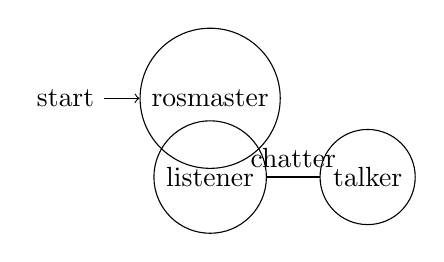
\begin{tikzpicture}
    % tikz code goes here
    \node[state, initial] (1) {rosmaster};
    \node[state, below of=1] (2) {listener};
    \node[state, below of=1, right of=2] at (1,0) (3) {talker};

    \draw   (2) edge[above] node{chatter} (3);
\end{tikzpicture}\\\\
To view this architecture in ros(for debugging and making sure everything is correct) run the command: \\
\textbf{rosrun rqt\_graph rqt\_graph}

\section{Turtlesim}
First lets start by running roslaunch command. The roslaunch command allows you to launch multiple nodes and the rosmaster with just one command.\\
example: \emph{roslaunch turtle\_motion turtle\_clean.launch} \\(remember to create the package as instructed in the ROS\_Instructions pdf available on blackboard.)\\\\
If nothing happens on the turtle simulator, open up the file catkin\_ws/src/turtle\_motion/src/grid\_clean.py and call any of the functions included from there in the main function.\\\\
This command will run your rosmaster, rosrun turtlesim turtlesim\_node, and rosrun turtle\_motion grid\_clean.py all in one terminal and you do not have to worry about managing multiple nodes across multiple terminals.\\\\
\begin{figure}[htp]
    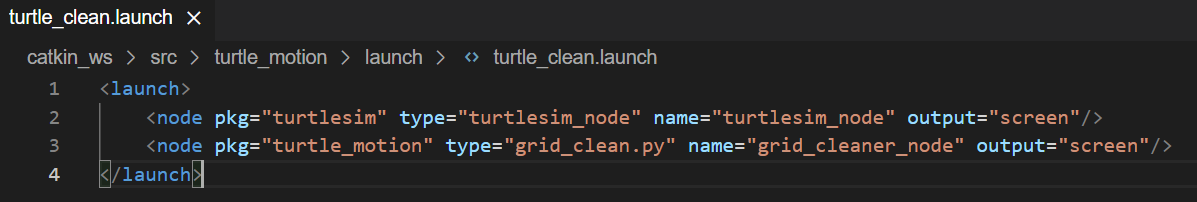
\includegraphics[width=12cm]{launchfile.png}
    \label{fig:launch}
\end{figure} \\
The important things to note about this file is that you must start and end the file with the launch tag ($<$launch$>$).  Each node you set up begins with a node tag($<$node$>$) and then you must specify the package where the node is contained(pkg=), the name of the file that sets up the node(type=), and the name of the node(name=); all other arguments are optional.
\newpage

\begin{figure}[htp]
    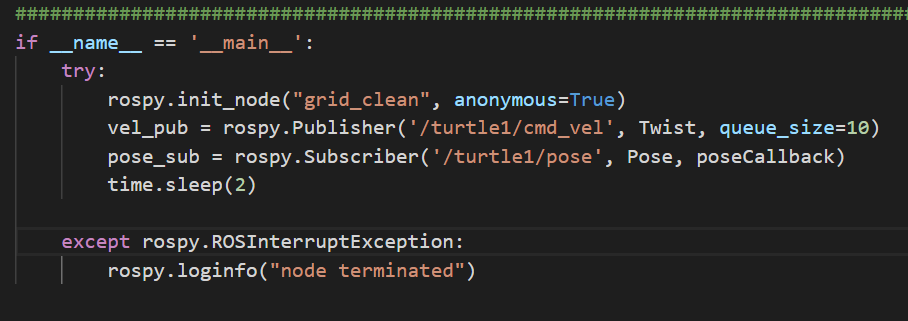
\includegraphics[width=12cm]{main.png}
    \label{fig:mainy}
\end{figure} \\
The image above shows how we set up the node, publisher and subscriber. Note that every time you set up a publisher or subscriber you must both provide a topic name and a message type.Example: rospy.Subscriber(topic\_name, msg\_type, callback function name). The callback function is written by the programmer, and it is the code that is executed every time the node receives a message on a topic.\\\\

\begin{figure}[htp]
    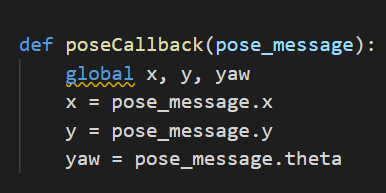
\includegraphics[width=10cm]{callback.png}
    \label{fig:callback}
\end{figure} \\
Example of callback in code that updates variables x, y, and yaw based on the robots current position on the simulator.\\\\
\newpage 

\begin{figure}[htp]
    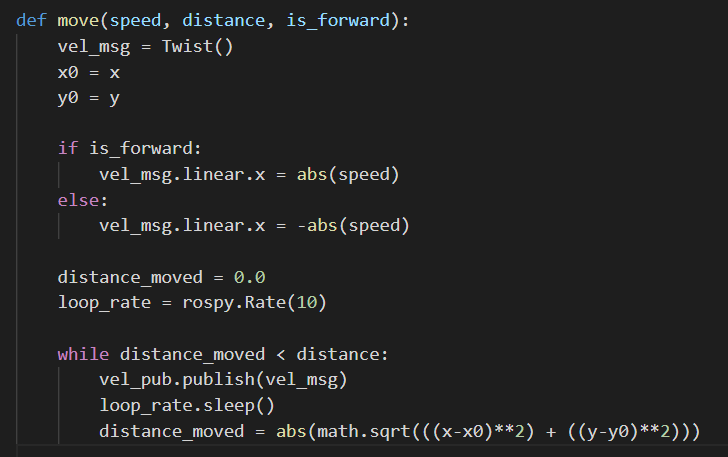
\includegraphics[width=10cm]{move.png}
    \label{fig:move}
\end{figure} \\
The move function has the robot move at some speed linear.x by publishing to the /turtle1/cmd\_vel topic. The message type of this topic is geometry\_msgs/Twist. This message has two member variables Vector3 linear and Vector3 angular. The linear variable sets the linear velocity of the turtle and the angular variable sets the angular velocity of the turtle robot. In the code we use the distance formula to compute how much the robot has moved from its initial position.\\\\

\begin{figure}[htp]
    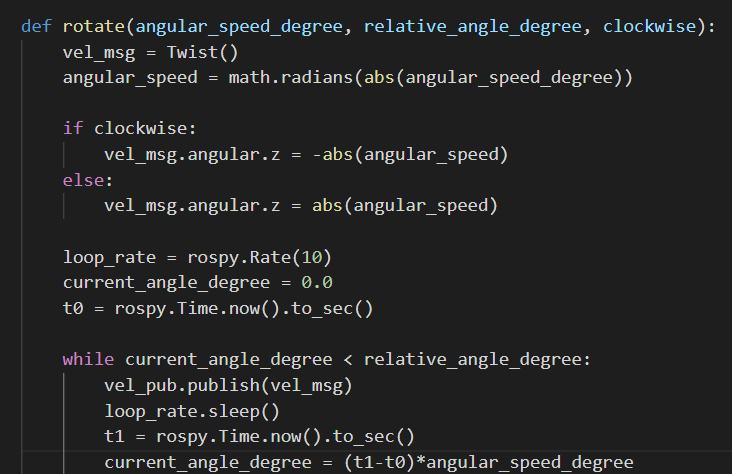
\includegraphics[width=10cm]{rotate.png}
    \label{fig:rotate}
\end{figure} \\
The rotate function also publishes /turtle1/cmd\_vel topic and uses a message type of geometry\_msgs/Twist. This time we are interested 
in the member variable Vector3 angular which sets the rotational velocity of the robot. The speed input parameter tells us how fast our turtle robot will rotate per second, and the idea is to rotate for however many seconds are required to reach our goal. 
\subsection{turtle architecture}
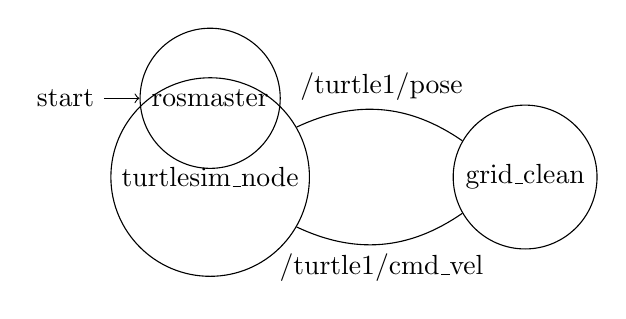
\begin{tikzpicture}
    % tikz code goes here
    \node[state, initial] (1) {rosmaster};
    \node[state, below of=1] (2) {turtlesim\_node};
    \node[state, below of=1, right of=2] at (3,0) (3) {grid\_clean};

    \draw   (2) edge[above] [bend left] node{/turtle1/pose} (3) 
            (3) edge[below] [bend left] node{/turtle1/cmd\_vel} (2);
\end{tikzpicture}

\newpage


\end{document}
